% --- 题目 ---
\problem[P18-1 (25-2)]{设函数 $\displaystyle f(x)$ 连续, 给出下列四个条件:
\\
\textcircled{1} $\displaystyle \lim_{x \to 0} \frac{|f(x)| - f(0)}{x}$ 存在;
\\
\textcircled{2} $\displaystyle \lim_{x \to 0} \frac{f(x) - f(0)}{x}$ 存在;
\\
\textcircled{3} $\displaystyle \lim_{x \to 0} \frac{|f(x)|}{x}$ 存在;
\\
\textcircled{4} $\displaystyle \lim_{x \to 0} \frac{|f(x)| - |f(0)|}{x}$ 存在.
\\
其中能得到 “$\displaystyle f(x)$ 在 $\displaystyle x=0$ 处可导” 的条件的个数是 ( \quad )
\begin{tasks}(4)
\task 1.
\task 2.
\task 3.
\task 4.
\end{tasks}}
\ansat{249;【十年真题】 - 考点:导数与微分的概念 - 1}

% --- 题目 ---
\problem[P18-7 (16-1)]{已知函数 $\displaystyle f(x) = \begin{cases} \displaystyle x, & \displaystyle x \le 0, \\ \displaystyle \frac{1}{n}, & \displaystyle \frac{1}{n+1} < x \le \frac{1}{n}, n = 1, 2, \dots, \end{cases}$ 则 ( \quad )}
\begin{tasks}(2)
\task $\displaystyle x=0$ 是 $\displaystyle f(x)$ 的第一类间断点.
\task $\displaystyle x=0$ 是 $\displaystyle f(x)$ 的第二类间断点.
\task $\displaystyle f(x)$ 在 $\displaystyle x=0$ 处连续但不可导.
\task $\displaystyle f(x)$ 在 $\displaystyle x=0$ 处可导.
\end{tasks}
\ansat{250;【十年真题】 - 考点:导数与微分的概念 - 7}

% --- 题目 ---
\problem[P18-8 (25-2,3)]{设函数 $\displaystyle f(x)$ 在 $\displaystyle x = 0$ 处连续, 且 $\displaystyle \lim_{x \to 0} \frac{x f(x) - \mathrm{e}^{2\sin x} + 1}{\ln(1+x) + \ln(1-x)} = -3$, 证明 $\displaystyle f(x)$ 在 $\displaystyle x=0$ 处可导, 并求 $\displaystyle f'(0)$.}
\ansat{250;【十年真题】 - 考点:导数与微分的概念 - 8}

% --- 题目 ---
\problem[P18-9 (22-2)]{已知函数 $\displaystyle f(x)$ 在 $\displaystyle x=1$ 处可导, 且 $$\displaystyle \lim_{x \to 0} \frac{f(\mathrm{e}^{x^2}) - 3f(1 + \sin^2 x)}{x^2} = 2,$$ 求 $\displaystyle f^{\prime}(1)$.}
\ansat{250;【十年真题】 - 考点:导数与微分的概念 - 9}

% --- 题目 ---
\problem[P20-1 (07-1,2,3)]{设函数 $\displaystyle f(x)$ 在 $\displaystyle x=0$ 处连续, 下列命题错误的是 ( \quad )
\begin{tasks}(2)
\task 若 $\displaystyle \lim_{x \to 0} \frac{f(x)}{x}$ 存在, 则 $\displaystyle f(0)=0$.
\task 若 $\displaystyle \lim_{x \to 0} \frac{f(x)+f(-x)}{x}$ 存在, 则 $\displaystyle f(0)=0$.
\task 若 $\displaystyle \lim_{x \to 0} \frac{f(x)}{x}$ 存在, 则 $\displaystyle f'(0)$ 存在.
\task 若 $\displaystyle \lim_{x \to 0} \frac{f(x)-f(-x)}{x}$ 存在, 则 $\displaystyle f'(0)$ 存在.
\end{tasks}}
\ansat{250;【真题精选】 - 考点:导数与微分的概念 - 1}

% --- 题目 ---
\problem[P20-3 (05-1,2)]{设函数 $\displaystyle f(x) = \lim_{n \to \infty} \sqrt[n]{1+|x|^{3n}}$, 则 $\displaystyle f(x)$ 在 $\displaystyle (-\infty, +\infty)$ 内 ( \quad )}
\begin{tasks}(2)
\task 处处可导.
\task 恰有一个不可导点.
\task 恰有两个不可导点.
\task 至少有三个不可导点.
\end{tasks}
\ansat{251;【真题精选】 - 考点:导数与微分的概念 - 3}

% --- 题目 ---
\problem[P21-9 (03-3)]{设函数 $\displaystyle f(x) = \begin{cases} \displaystyle x^\lambda \cos \frac{1}{x}, & \displaystyle x \neq 0, \\ \displaystyle 0, & \displaystyle x=0, \end{cases}$ 其导函数在 $\displaystyle x=0$ 处连续, 则 $\displaystyle \lambda$ 的取值范围是 \underline{\hspace{4em}}.}
\ansat{251;【真题精选】 - 考点:导数与微分的概念 - 9}

% --- 题目 ---
\problem[P21-2 (22-2)]{已知函数 $\displaystyle y=y(x)$ 由方程
\[ x^2 + xy + y^3 = 3 \]
确定, 则 $\displaystyle y''(1) = \underline{\hspace{4em}}. $}
\ansat{251;【十年真题】 - 考点一:函数的求导与微分法则 - 2}
\vspace{12em}

% --- 题目 ---
\problem[P21-1 (21-1)]{设函数 $\displaystyle f(x)=\frac{\sin x}{1+x^2}$ 在 $\displaystyle x=0$ 处的 3 次泰勒多项式为 $\displaystyle ax+bx^2+cx^3$, 则 ( \quad )}
\begin{tasks}(2)
\task $\displaystyle a=1, b=0, c=-\frac{7}{6}$.
\task $\displaystyle a=1, b=0, c=\frac{7}{6}$.
\task $\displaystyle a=-1, b=-1, c=-\frac{7}{6}$.
\task $\displaystyle a=-1, b=-1, c=\frac{7}{6}$.
\end{tasks}
\ansat{251;【十年真题】 - 考点二:高阶导数的计算 - 1}

% --- 题目 ---
\problem[P21-7 (16-1)]{设函数 $\displaystyle f(x) = \arctan x - \frac{x}{1+ax^2}$, 且 $\displaystyle f'''(0) = 1$, 则 $\displaystyle a = \underline{\hspace{4em}}. $}
\ansat{251;【十年真题】 - 考点二:高阶导数的计算 - 7}

% --- 题目 ---
\problem[P24-例(2)]{设函数 $\displaystyle y=x^2 \sin 2x$, 则 $\displaystyle y^{(5)}(0) = \underline{\hspace{4em}}. $}
\ansat{24;【方法探究】 - 考点二:高阶导数的计算 - 例(2)}

% --- 题目 ---
\problem[P25-7 (97-3)]{设 $\displaystyle y = f(\ln x) \mathrm{e}^{f(x)}$, 其中 $\displaystyle f$ 可微, 则 $\displaystyle \mathrm{d}y = \underline{\hspace{4em}}. $}
\ansat{252;【真题精选】 - 考点一:函数的求导与微分法则 - 7}

% --- 题目 ---
\problem[P26-2 (20-3)]{曲线 $\displaystyle x + y + \mathrm{e}^{2xy} = 0$ 在点 $\displaystyle (0, -1)$ 处的切线方程为 $\underline{\hspace{4em}}.$}
\ansat{254;【十年真题】 - 考点一:平面曲线的切线与法线 - 2}

% --- 题目 ---
\problem[P26-1 (23-2)]{设函数 $\displaystyle f(x)=(x^2+a)\mathrm{e}^x$. 若 $f(x)$ 没有极值点, 但曲线 $y=f(x)$ 有拐点, 则 $a$ 的取值范围是 ( \quad )}
\begin{tasks}(2)
  \task $\displaystyle [0,1).$
  \task $\displaystyle [1, +\infty).$
  \task $\displaystyle [1, 2)$
  \task $\displaystyle [2, +\infty).$
\end{tasks}
\ansat{254;【十年真题】 - 考点二:利用导数判断函数的性质 - 1}

% --- 题目 ---
\problem[P26-2 (22-2)]{设函数 $\displaystyle f(x)$ 在 $\displaystyle x=x_0$ 处具有 2 阶导数, 则 ( \quad )}
\begin{tasks}(1)
  \task 当 $\displaystyle f(x)$ 在 $\displaystyle x_0$ 的某邻域内单调增加时, $\displaystyle f'(x_0)>0$.
  \task 当 $\displaystyle f'(x_0)>0$ 时, $\displaystyle f(x)$ 在 $\displaystyle x_0$ 的某邻域内单调增加.
  \task 当 $\displaystyle f(x)$ 在 $\displaystyle x_0$ 的某邻域内是凹函数时, $\displaystyle f''(x_0)>0$.
  \task 当 $\displaystyle f''(x_0)>0$ 时, $\displaystyle f(x)$ 在 $\displaystyle x_0$ 的某邻域内是凹函数.
\end{tasks}
\ansat{254;【十年真题】 - 考点二:利用导数判断函数的性质 - 2}

% --- 题目 ---
\problem[P26-4 (19-1)]{设函数 $\displaystyle f(x)=\begin{cases} x|x|, & x \le 0, \\ x\ln x, & x > 0, \end{cases}$ 则 $\displaystyle x=0$ 是 $\displaystyle f(x)$ 的 ( \quad )}
\begin{tasks}(2)
  \task 可导点, 极值点.
  \task 不可导点, 极值点.
  \task 可导点, 非极值点.
  \task 不可导点, 非极值点.
\end{tasks}
\ansat{254;【十年真题】 - 考点二:利用导数判断函数的性质 - 4}

% --- 题目 ---
\problem[P26-5 (16-2,3)]{设函数 $\displaystyle f(x)$ 在 $\displaystyle (-\infty, +\infty)$ 内连续, 其导函数的图形如下图所示, 则 ( \quad )
\begin{center}
    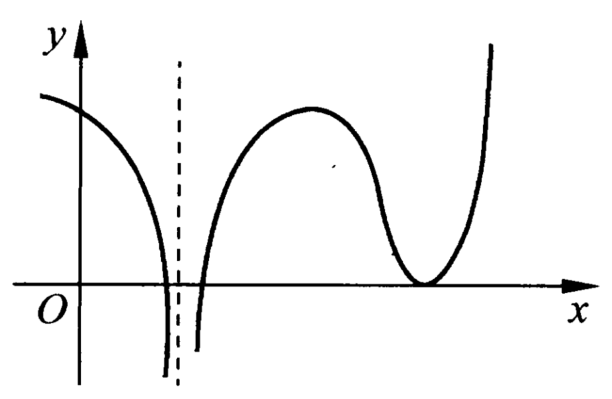
\includegraphics[width=0.5\textwidth]{P26-5_16-2_3.png} % 
\end{center}
\begin{tasks}(1)
  \task 函数 $\displaystyle f(x)$ 有 2 个极值点, 曲线 $\displaystyle y=f(x)$ 有 2 个拐点.
  \task 函数 $\displaystyle f(x)$ 有 2 个极值点, 曲线 $\displaystyle y=f(x)$ 有 3 个拐点.
  \task 函数 $\displaystyle f(x)$ 有 3 个极值点, 曲线 $\displaystyle y=f(x)$ 有 1 个拐点.
  \task 函数 $\displaystyle f(x)$ 有 3 个极值点, 曲线 $\displaystyle y=f(x)$ 有 2 个拐点.
\end{tasks}}
\ansat{254;【十年真题】 - 考点二:利用导数判断函数的性质 - 5}

% --- 题目 ---
\problem[P26-6 (19-2,3)]{曲线 $\displaystyle y = x \sin x + 2 \cos x \ \left(-\frac{\pi}{2} < x < \frac{3\pi}{2}\right)$ 的拐点坐标为 $\underline{\hspace{4em}}.$}
\ansat{254;【十年真题】 - 考点二:利用导数判断函数的性质 - 6}

% --- 题目 ---
\problem[P26-9 (21-2)]{已知函数 $\displaystyle f(x) = \frac{x|x|}{1+x}$, 求曲线 $\displaystyle y=f(x)$ 的凹凸区间及渐近线.}
\ansat{254;【十年真题】 - 考点二:利用导数判断函数的性质 - 9}